In this chapter we finally arrive to our main interest. First of all we introduce the hierarchy of data structures with respect to persistence.

\begin{itemize}
\item {\bfseries Ephemeral data structures} are the most widespread. 
Past states are destroyed by "destructive" updates and irretrievably lost.
\item {\bfseries Semi-persistent data structures} (sometimes partially persistent) 
still support modifying operations only on the most recent version. 
Updates produce a new version of the structure. 
Historical versions form a linear order. 
Past states can be reconstructed efficiently for reading.
\item {\bfseries (Fully-)persistent data structures} directly extend their semi-persistent counterparts. 
An update can be done on any version of the structure, resulting in a rooted tree of versions. 
An update corresponds to adding a new child vertex to an existing vertex in the tree.
\item {\bfseries Functional data structures} permit no changes to data once written. 
Naturally, persistence is guaranteed under such an assumption, 
as all versions appear as if just created by the last update.
This enforced immutability completely freezes past version in time.
This concept is intrinsic to functional languages such as Haskell, 
but proves to be useful even in imperative programming. 
Multi-threading is easier when there is confidence that existing objects will not be modified.
\end{itemize}.

This division is by no means universally adopted, but provides an interesting perspective regardless.

With a persistent data structure, we essentially want to have one data structure for every existing version. Insert and delete return a new version handle instead of making changes to the existing version. Obviously, copying the data structure every time is one option how to achieve this, albeit not a great one. To prevent using extra memory and increased time complexity of operations however, more intricate methods must be employed.

Going beyond this hierarchy, if fully-persistent data structure also supports merging or melding two different versions, it is said to be \emph{confluently persistent}. Confluently persistent data structures are the subject of studies for example by Driscoll, Sleator, and Tarjan\cite{confluently-persistent-a} or Fiats and Kaplan\cite{confluently-persistent-b}. We will not investigate confluent persistence in this thesis further.

\section{Persistence through Path-Copying}

Let us open with a few simple constructions first. Binary search tree can be converted into a fully-persistent one rather easily.
The straight-forward approach is called path-copying. It is based on the observation that most of the tree does not change during an update.

When a new version of the tree should by created by delete or insert, new copies are allocated only for vertices that are changed by the operation and their ancestors. 
This typically means that only path from the inserted/deleted vertex to the root is newly allocated, plus constant number of other vertices. 
The new vertices carry pointers to the old vertices where subtree rooted at such a vertex is not modified in any way.
Here we tacitly assume that only pointers to children are stored. Updating root in a tree with pointers to parents would involve creating new instances for all nodes in the tree.

With reasonable variants of binary search trees, achieved time complexity in a tree with $n$ vertices is $\Theta(\log n)$ per operation and $\Theta(\log n)$ memory for insert/delete.

The downside of this method is the increased space complexity. There is no apparent construction that would not increase memory complexity by copying the paths.

\section{Multiple versions in one vertex}

To limit memory consumption we may rather choose to let vertices carry their properties for all versions. This in reality means that we must store a collection of changes together with versions when those changes happened. This makes a vertex a kind of dictionary with keys being versions and values the descriptions of changes.

When semi-persistence is sufficient, upon arriving at a vertex asking for the state in version $A$, we do the following: We must go through the collection of changes to figure out what the state in version $A$ should be. 
We start with the default values and apply all changes that happened earlier than $A$ in chronological order overwriting if there are multiple changes for the same field or pointer. 
This process yields the correct state of the vertex for version $A$. 

In fact, it might be easier to just copy all of the other fields the vertex possesses as well if one of them changes.
One change will therefore hold new values for all fields and pointers of the vertex. 

For full-persistence we also need to resolve the issue of how to effectively determining which changes should be applied. 
It will be addressed later through introduction of total ordering of all versions.

Looking at the memory consumption, it appears clear that the amount consumed stems from the total number of changes done by the balancing algorithm across all operations.

What remains to solve though is to choose the right kind of collection for versions of changes for one vertex. Surely using linked lists or arrays will inevitably lead to unsatisfactorily inefficient processing of applicable changes. Unfortunately as it turns out, even other data structures will let us down here.

With this approach, we can reach space complexity that is linear with the total number of changes in the tree. On the other hand execution time will be hurt. We can reach the following amortized complexity depending on the chosen data structure:

\begin{tabular}{ll}
Linked list & \bigO{n \log n} \\
Binary search tree & \bigO{\log^2 n} \\
Q-fast trie \cite{q-fast-trie} & \bigO{\log ^{3/2} n}, semi-persistence only \\
Y-fast trie \cite{y-fast-trie} & \bigO{\log n \cdot \log \log n}, semi-persistence only, on average

\end{tabular}

\begin{figure}
	\begin{center}
		\begin{tikzpicture}[sibling distance=8pt]
		\Tree[
		.B A [ .C \edge[blank]; \node[blank]{}; D ]
		]
		\node at (0,1) {Version 1};
		\end{tikzpicture}
		\qquad\hspace{40mm}
		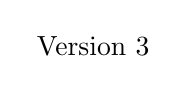
\begin{tikzpicture}[sibling distance=8pt]
		\Tree[
		.B A [ .D C E ]
		]
		\node at (0,1) {Version 3};
		\end{tikzpicture}
	\end{center}
\raggedcolumns
\begin{multicols}{2}
\centering
\footnotesize
\begin{vdTable}{Vertex}
	Version & Left & Right   & Key & Value
\end{vdTable}
\begin{vdTable}{A}
	1 & $\Lambda$ & $\Lambda$ & 10 & 5 \\
	2 & $\Lambda$ & $\Lambda$ & 10 & 6
\end{vdTable}
\begin{vdTable}{B}
	1 & A & C & 20 & 15 \\
	3 & A & D & 20 & 15
\end{vdTable}
\begin{vdTable}{C}
	1 & $\Lambda$ & D & 30 & 27 \\
	3 & $\Lambda$ & $\Lambda$ & 30 & 27
\end{vdTable}
\begin{vdTable}{D}
	1 & $\Lambda$ & $\Lambda$ & 40 & 39 \\
	3 & C & E & 40 & 39
\end{vdTable}
\begin{vdTable}{E}
	3 & $\Lambda$ & $\Lambda$ & 50 & 99
\end{vdTable}\\
\end{multicols}

{\small
Tree is shown for version 1 (left) and 3 (right). 
Internal collections for each vertex are displayed. 
Operation that created version 2 changed value of key 10. Operation that created version 3 inserted vertex E and triggered a rotation. 
Faithful to The Art of Computer Programming, $\Lambda$ represents a null pointer.
}

\caption{A tree with dictionaries in vertices} 

\end{figure}

\section{Fat Vertices}

Following up on the idea of multiple versions in one vertex, fat vertices were devised. 
We will explain this technique only for semi-persistence first. 
Full persistence requires the use of a few extra tricks and establishing an ordering on the versions.

A fat vertex stores a dictionary of standard vertices indexed by versions. 
We call values of this dictionary slots. 
The maximum size of this dictionary is set to a constant which is to be determined later. 
Temporarily, we will allow the capacity of fat vertex to be exceeded. 
This will have to be fixed however, before the ongoing operation finishes.
By placing a restriction on the size we may circumvent the increased complexity of search within one vertex.
Instead of copying the vertex, we simply add new slot into the dictionary. 
Provided the maximum has not been exceeded yet, this insertion of a slot stops the propagation of changes toward the root. 
The Reader should recall that this was the major weakness of path-copying.
Because of the limit on size of this dictionary, it may be implemented simply as a linked list.

Contents of one slot are a version handle, all pointers a vertex would have, then inverse pointers to fat vertices that have slots pointing to this fat vertex for this version and some fields, notably key and value as a bare minimum.
Not all fields need to be versioned. 
For example balancing information may be stored only for the latest version, i.e. in red-black trees color is only used for balancing and is thus not needed to be persisted for old versions. 
(Until full-persistence comes into play.)

One vertex in the original binary search then corresponds to a doubly-linked list of fat vertices.
When the vertex changes, new state of the vertex is written into a slot of the last fat vertex in the list. 
As all slots become occupied in the last fat vertex and it needs to be modified, new vertex is allocated.

Modifications of a single vertex during one operation are all written to single slot, there is no need for using more slots.

When a new fat vertex $x$ is allocated, one of its slots is immediately taken. 
Pointers must be updated in other fat vertices that pointed to the fat vertex preceding $x$ in the list. 
This is done either by inserting new slot into them (copying all values from the latest slot and replacing pointers to the predecessor by pointers to $x$). 
Or by directly updating the pointers if the right version is already present. 

Recursive allocations may be triggered, which is not a problem if there is only a small amount of them. 
This is ensured by setting the size of fat vertices suitably. 
The order in which these allocations are executed can be arbitrary.
We can place an upper bound on the number of newly allocated fat vertices -- total number of vertices in the tree (including deleted vertices). 
At most one new slot is occupied for every vertex in the tree.

To take advantage of fat vertices, we need the balancing algorithm to limit the number of vertices that change in one operation. 
This was the goal of modified WAVL-balancing algorithm all along. 
Furthermore, we need a limit on the number of pointers that can target one vertex at one time.

\begin{prop}
Suppose any binary search tree balancing algorithm satisfying the following properties:
\begin{itemize}
\item 
There is a constant $k$ such that for any $n$ successive operations on initially empty tree, the number of vertex changes made to the tree is at most $kn$. 
\item 
There is a constant bound on the number of pointers to any one vertex at any time.
\end{itemize}
Then this algorithm with the addition of fat vertices for semi-persistence, consumes \bigO{n} space for the entire history of $n$ operations starting from an empty tree.
\end{prop}

\begin{myproof}
We denote the number of pointer fields per vertex as $p$ and maximum number of vertices pointing to one vertex at a time as $x$. We then define the number of slots in fat vertex as $s = p + x + 1$. (Higher value is also possible)\\
We define the potential of the structure as the total number of occupied slots in all fat vertices that are the last in their doubly-linked list. (Thus initially zero.) Allocation of a new fat vertex will cost one unit of energy. This cost can be charged from the potential or the operation. We will show that the operation needs to be charged only a constant amount of energy per one vertex modification by the original algorithm (to compensate increase in potential or pay for allocations), from which the proposition follows.\\
For insert, a new vertex is created (which increases potential by a constant). During rebalancing of the tree, $r$ vertices are to be modified. Let us consider this sequence of modifications one by one. We send one floating unit of energy to each of the $r$ vertices.\\
If a modification of $v$ is second or later modification of $v$ during this operation, changes are simply written to the slot for this version.\\
Otherwise, number of used slots is checked. If there is one or more empty available, new slot is used, taking default values of fields from preceding slot. This increases potential by one, which is covered by the floating unit of energy.\\
If no slots are available, new fat vertex $v'$ is allocated and one of its slots is used. This step triggers a decrease in the potential by $p+x$. The floating unit of energy is used to pay for allocation of the new vertex. Next, fat vertices to corresponding current version interval of vertices having pointers to $v$ need to have this reflected. Additionally inverse pointers to $v'$ need to be set. These are at most $p+x$ changes to other vertices that may use their new empty slots. The decrease in potential is used to send one unit of energy to every such vertex that need an update. Changes are executed recursively and will not require extra energy to be charged on this modification.
\end{myproof}

Regarding the time complexity, searching the correct slot in a fat vertex produces only constant overhead. Realizing that every operation can be charged on a memory allocation of a fat vertex such that there is a constant $c$ depending only on the balancing algorithm such that for every allocated fat vertex the number of operations charged on it is at most $c$.

\begin{obs}
Assuming the conditions from the previous proposition, the cost to write changes into fat vertices is amortized to \bigO{1} per operation.
\end{obs}

We see that WAVL trees can be used for semi-persistence even in their original form, along with many other binary search trees. Time complexity of operations with the tree depends on the original balancing algorithm used. With WAVL trees we get \bigO{\log n} per operation from the original algorithm in addition to the amortized \bigO{1}. Here $n$ is the size of the tree in the version that is queried.

In fact, for semi-persistence fat vertices may be defined differently. It suffices that only values of changed fields and pointers are written into slots. Thus each fat vertex carries a set of default values for every field and pointer, these values are used if not overridden by a slot. This approach may lead to lower memory consumption and is not directly compatible with the approach to full persistence described later.

\begin{figure}
\begin{center}
	\ttfamily
	\begin{tabular}{cccccc}
		Rank  & Previous &  Next   &      & &          \\ \hline
		Left1 &  Right1  & Parent1 & Key1 & Value1 &  Version1 \\ \hline
		Left2 &  Right2  & Parent2 & Key2 & Value2 & Version2 \\ \hline
		Left3 &  Right3  & Parent3 & Key3 & Value3 & Version3 \\ \hline
		Left4 &  Right4  & Parent4 & Key4 & Value4 & Version4 \\ \hline
		Left5 &  Right5  & Parent5 & Key5 & Value5 & Version5 \\ \hline
		Left6 &  Right6  & Parent6 & Key6 & Value6 & Version6 \\ \hline
	\end{tabular}
\end{center}
Rank of WAVL trees is not used for navigation only for balancing the tree, it need not be maintained for older versions.
\caption{Layout for WAVL semi-persistent tree fat vertex}
\end{figure}

\section{Parallel Semi-Persistence with WAVL Trees}

Recall that insertion and deletion in a WAVL tree can be also carried out top-down.
By preemptively performing rotations, promotes and demotes when descending, we can make sure that large number of changes of vertices with high ranks will not be needed. This means that as insert or delete will descend down the tree towards the leaves processing vertices along some vertical path, it will hold locks for vertices in at most constant distance from the vertex that the operation is currently processing.

Also recall that there are at most \bigO{1} modifications of the structure per update (amortized), albeit the constant proves to be rather high. These facts lay a solid foundation to parallel semi-persistence.

What seems a bit unfortunate, is the delete procedure, which must locate an additional vertex to swap values in case of the deleted vertex having two children. So we will assume that delete is not possible for now.

First of all two kinds of supported operations must be identified. 

\begin{itemize}
	\item Query on any version of the tree (id est find, min, max and range functions)
	\item Insert (into the newest version of the tree)
\end{itemize}

Let us address data races between inserts first. For every insert, prior to all else, new version handle must be created. This is achieved simply by incrementing a version counter which is done by a primitive such as fetch-and-add and will not block other threads. The insert itself follows.

Locking procedure will be this: When we enter a fat vertex, we lock it for other threads of computation. Conversely, a lock for a fat vertex is lifted when it ceases to be in the subtree of current safe-node's parent for insert holding the lock. Since all threads begin locking at the root and descend towards the leaves, no deadlocking is possible among inserts. This follows from the fact that rotations may only done among vertices locked by the same operation.

Applying the algorithm with semi-persistence we must additionally ensure that before unlocking a fat node, none of its children may run out of slots leading to allocation of a replacement. Since there can be at most one new slot occupied for every fat node in one operation, it suffices to allocate new fat vertex for every fat vertex without empty slots before releasing its parent. This may involve increasing the capacity of fat vertices.

To ensure that the most most recent fat vertex for root does not change after some operation starts waiting for the lock for access to it, we introduce additional \emph{latest-root} pointer to the current latest fat vertex of the root. 

When some update changes the fat vertex that corresponds to the root, it updates this pointer. New updates start by waiting for lock for this pointer. This lock is lifted when the holding operation wows not change root of the tree.

To address queries, we assume that queries are only started on a version that was generated by already complete insert. In this situation, queries may pass through fat vertices with little regard to ongoing inserts. Queries will thus ignore locks on fat vertices. Only one thing must be considered -- modification of slots by insert (being non-atomic) requires exclusive write lock on the slots that are modified. Queries will require shared read-only lock. Since reading of information from slots by insert may only be obstructed by writing by the same insert, read-only lock is not needed in this case. No deadlocks will arise from this locking can be conducted starting from the head of slots linked list in all cases. 

Alternatively, version of slots might be set atomically by operations as the last field to be set in creation the slot. Query operations might check version of a slot first and if it equals the default value, assume that it is not yet occupied. This would indicate that all remaining slots are also empty. The query would thus know it does not need the information stored in those slots and proceed as if those did not exist.

If we increase the number of slots in a fat vertex by at least one, asymptotic memory consumption remains linear with length of history. Time complexity for one operation remains the same as without this modification for concurrence, that is if time spend being blocked by other threads is excluded.

Let us turn back to enabling delete. If delete operations are rare, we may simply treat them as inserts locking-wise and acknowledge that blocking may ensue. Another approach would be to use the technique of \textit{ghost vertices}. That is to add a deleted flag to vertex layout, deleting would simply set this flag in corresponding slot. This will increase size of the tree. For the number of deleted vertices bounded by a polynomial in the number of remaining vertices for every version of the data structure, this preserves the asymptotic time complexity. 

Otherwise, an entirely new data structure may be built from the latest versions of all vertices in the tree if the amount of deleted vertices exceeds a certain ratio to remaining vertices. The cost to build this new tree is amortized into the deletes from the preceding data structure.

\begin{figure}
	\begin{center}
		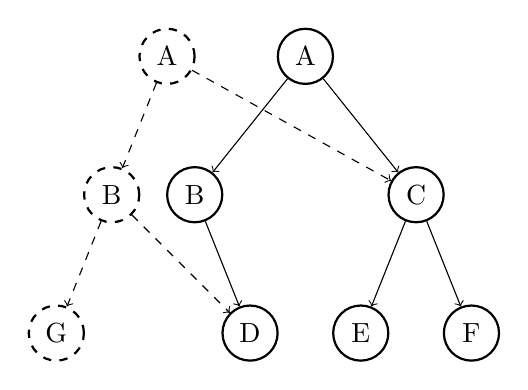
\begin{tikzpicture}[
			oldnode/.style={circle, draw=black, thick, minimum size=7mm},
			newnode/.style={circle, thick, draw=black, dashed, minimum size=7mm},
			]
			\node[oldnode] at (0,0) (root) {A};
			\node[oldnode] at (-4em,-5em) (beta) {B};
			\node[oldnode] at (4em,-5em) (gamma) {C};
			\node[oldnode] at (-2em,-10em) (delta) {D};
			\node[oldnode] at (2em,-10em) (epsilon) {E};
			\node[oldnode] at (6em,-10em) (zeta) {F};
			\node[newnode] at (-5em,0) (newroot) {A};
			\node[newnode] at (-7em,-5em) (newbeta) {B};
			\node[newnode] at (-9em,-10em) (newvertex) {G};
			\draw[->] (root) -- (beta);
			\draw[->] (root) -- (gamma);
			\draw[->] (beta) -- (delta);
			\draw[->] (gamma) -- (zeta);
			\draw[->] (gamma) -- (epsilon);
			\draw[->,dashed] (newroot) -- (gamma);
			\draw[->,dashed] (newroot) -- (newbeta);
			\draw[->,dashed] (newbeta) -- (newvertex);
			\draw[->,dashed] (newbeta) -- (delta);
		\end{tikzpicture}
	\end{center}
	A new vertex G was added to the structure with solid vertices. Dashed vertices were created by the update -- path from G to the root. Dashed A is the new root.
	\caption{Path-copying}
	\label{fig:path-copying}
\end{figure}

\section{List Ordering}

Moving from semi-persistence to full-persistence we encounter an obstacle -- versions no longer form implicit linear order. (By versions we mean states of the tree in between updates. We will also use some auxiliary versions not directly mappable to any such state.) Nonetheless, to work with fat vertices, we need to be able to determine slots that carry values correct for current version. To achieve this, we need to identify an interval of versions the current vesion would fall into. For this purpose we will try to introduce an ordering to versions of the persistent data structure.

Version do form a rooted tree with the original version in the root. We can also order children of every vertex by the order of their creation (latest creation first). We then define the desired ordering as the order of vertices corresponding to versions as they are visited by an in-order traversal. %TODO: Reformulate in-order.

In reality, we will also insert other elements into the ordering that will be helper version and will not be used to represent the state of the entire structure after a sequence of operations. This can be disregarded for now.

With the ordering defined, we still need a way to efficiently represent it in memory. The operations we really need are two:

\begin{itemize}
	\item \texttt{InsertSuccessor(Version)} -- this operation will insert a new version between \texttt{Version} and its successor (if any). The newly created version is returned.
	\item \texttt{Compare(VersionA, VersionB)} -- returns 1, $-1$, or 0 indicating whether \texttt{VersionA} precedes, succeeds, or equals \texttt{VersionB}.
\end{itemize}

We will strive to find a way to assign an integer to each version, these integers will be comparable in constant time. This assignment problem is called \emph{list-labeling} and there are several options to tackling it.

The straight-forward idea would be to assign 0 to the first version and $2^m$ to an artificial upper bound. All newer versions will be assigned the arithmetic average of its successor and predecessor. Now, we see that if $v = (p + s)/2$ and $ 2^k \mid p, s$, then $2^{k-1} \mid v$. The first two integers are divisible by $2^m$ guaranteeing capacity $\Omega(m)$. 

Let us denote the total number of updates to the persistent tree as $n$. It would be reasonable to  assume that arithmetic operations on non-negative integers less than or equal to $n$ can be done in constant time. We are therefore permitted to create only \bigO{\log n} versions using the straight-forward idea if constant time per operation is needed. This is not sufficient.

To preserve the speed of semi-persistence, \texttt{Compare} must be \bigO{1} and \texttt{InsertSuccessor} \bigO{\log n} at least amortized. Weight-balanced trees that were introduced in the previous chapter are ideally suited for this purpose.

For every vertex in the weight-balanced tree, we will store encoding of the path from root to it in form of sequence of 0s and 1s. 1 for right child, 0 for left child. We know that depth of the tree must be logarithmic, compared integers are composed of \bigO{\log n} bits, so comparison of versions is efficient. Inserting a successor version is also simple. Rebuilding of some subtree will not change order of versions as all path encodings will be recalculated.

Before moving to the next section, we remark that it is possible to get \bigO{1} amortized complexity for insert and delete with weight-balanced trees via indirection as described by Tsakalidis \cite{list-ordering}.

\section{Fully-Persistent Trees}

Before delving into the details of modified fat vertices for full-persistence, we must note that amortized constant number of changes per operation will no longer suffice. If there exist a version of the structure and an operation that causes large amount of changes to the structure, nothing is stopping us from repeatedly performing this operation on this version, thus consuming super-linear amount of space.

For achieving full persistence, we will build upon the technique of fat vertices. Now however, simply allocating new vertex when we run out of empty slots in the old one will not do. It remains crucial that occupied slots of one fat vertex form an interval of existing versions. In particular, It will be needed to insert between existing versions.

A new maximum size $m$ of fat vertices will have to be set. If $p$ is the number of pointer fields in original vertices and $k$ the number of required inverse pointers, we set $m = 4(p+k+1)$.
When searching a fat vertex, the slot that applies has the greatest version not exceeding the version that is currently being searched for.


A process modifying the BST data structure may be broken down into a series of updates that only change one vertex. (Or insert a new one.)
Every such update of the data structure will produce a new version (more than one actually). since were are only interested in the versions that are associated with the modification that completed an operation on the data structure, existence of other versions can be safely ignored. The total number of versions created will still be in $O(\# operations)$, preserving time complexity.

The process of performing one update involves first of all locating the slot that will be updated. If there exists a slot with the exact same version $v$, it will be updated. Otherwise the slot $s$ corresponding to $v$ is located and copied twice, creating $s'$ and $s''$. $s'$ is given the version $v$ and $s''$ a newly created version that succeeds $v$. Then values in $s'$ are updated.
If the update is insert a new fat vertex with one slot is created instead and its field and pointer values are initialized.
If the current fat vertex has exceeded the number of permitted slots, we add it to a list $l$.
Now inverse pointers must be set in other fat vertices. Similarly, if a slot matching the version is already present there modifications are applied to that slot. Otherwise two other slots are inserted just as already described. In addition, we add any of the fat vertices where inverse-pointers were updated and slot-capacity exceeded to $l$.

During the update, we must make sure that the number of slots in one fat vertex does not exceed $m$ by too many. We assure this by processing the fat vertex with the most slots filled next. Since we have placed a limit on the number of new slots added by one node-splitting and it cannot add more than one slot to a vertex, we can limit the highest obtainable amount of slots in one vertex by a constant multiple of $m$.

We therefore maintain $l$ as an array of linked lists indexed by sizes of those fat vertices. When we add to $l$, we append to the linked list with the adequate size. When the size changes, the outdated records remain in the linked-lists. Therefore, when extracting from $l$ we must first check that the size is still valid, if another extract is performed until a valid item is found or all lists are empty. As we add only constant amount of items to $l$ per node-splitting, the overall time spent extracting next vertex from $l$ is linear with the amount of node-splittings and need not be analysed further.

Now while $l$ is nonempty we take a fat vertex $f$ with the highest size from it, check that the number of slots contains was exceeds the limit and then split the node in two. This means allocating a new fat vertex $f'$ and placing half of the slots with higher versions in it. After this split, another pointer check is needed. For versions in the higher half of slots (now slots of $f$), regular and inverse pointers must be checked. For every slot in other fat vertex corresponding to a version belonging to $f'$  that has pointers to $f$, these must be changed to $f'$. 

One slight problem is that the interval might overlap with version from both $f$ and $f'$, in that case a slot with lowest version belonging to $f'$ must be inserted, copying the preceding slot in fields and pointers not to $f$. We know however, that this overlapping can only happen for vertices pointed to by both the slot with greatest version in $f$ and lowest version in $f'$. This insert may cause the permitted number of slots to be exceeded and if that is the case, this fat vertex must be appended to $l$.

Now it is in order to show that $l$ will eventually become empty and what the time complexity is.

\begin{prop}
Starting with an initially empty fully-persistent binary search tree data structure (as described above), a sequence of $n$ updates produces a data structure taking \bigO{n} space while taking \bigO{n \log n} time.
\end{prop}

\begin{proof}
Let us define a potential function for a persistent BST as the sum over all fat vertices of that structure of the number of occupied slots above $3m/4$. Initially the potential is zero and may never be negative. Every update will be charged $m/2 \in \mathcal{O}(1)$ units of energy.

During the first phase, i.e. writing actual changes in the tree to one node, at most $m/2$ extra slots become occupied, these are charged on the update.

During the phase when $l$ is processed, let us have a fat vertex $f$ in $l$. If the size of $f$ is exceeded we must allocate a new fat vertex $f'$. Distributing slots between the two vertices decreases potential by a least $m/4$. We use 1 unit to pay for the new allocation and the remaining units to pay for increase in potential during the check for (inverse-)pointer validity, that is inserting of slots. This implies that potential of the data structure decreases by at least 1 for each splitting in the phase of $l$ processing.

From this argument we also see that the number of node-splitting occurring during one update is limited by the amount of potential available at the start of that update, so it must come to an end.

Every action is now accounted for and the proof is complete.
\end{proof}

\begin{cor}
A sequence of any $n$ tree-operations and $q$ queries on a fully persistent WAVL tree (initially empty) produces a data structure which consumes \bigO{n} memory and takes \bigO{(n+q) \log n} time.
\end{cor}

We should note that the size of vertices is so large, because we did not place any constraint on what updates are allowed to change. If update is only able to change one pointer field for example, we could reduce the size significantly. This would need to be analysed separately for each data structure.

%\begin{prop}
%Suppose any order of splitting fat vertices with the number of slots exceeding the set limit $l$ %during an operation on a tree $T$. Regardless of the way for choosing the next node to be split, %number of occupied slots in all nodes will remain under .
%\end{prop}

Finally, let us conclude this chapter with a remark that this approach may be generalized further beyond binary search trees to other pointer-based data structures provided that the constraint on number of pointers targeting one node simultaneously applies to them.
We do not give more attention to such structures in this thesis.
